\part{Teorie}

\chapter{Základní geometrické pojmy}
%úsečka, afinní množina, konvexní množina, ...

Mějme dva body $x_1, x_2 \in \mathbb{R}^n$ takové, že $x_1 \neq x_2$ a parametr $\theta \in \mathbb{R}^n$. Potom výraz
\begin{equation}
    y = \theta x_1 + (1 - \theta) x_2
    \label{line}
\end{equation}
popisuje \textbf{přímku} procházející body $x_1$ a $x_2$. Pro $\theta = 0$ dostáváme bod $x_2$ a pro $\theta = 1$ bod $x_1$. Omezíme-li tedy $\theta$ na interval $\langle 0, 1 \rangle$, dostaneme \textbf{úsečku} s koncovými body $x_1$ a $x_2$. Výraz \ref{line} lze přepsat do tvaru
$$
    y = x_2 + \theta (x_1 - x_2),
$$
který můžeme interpretovat jako součet počátečního bodu $x_2$ a nějakého násobku směrového vektoru $x_1 - x_2$.

\noindent Říkáme, že $C \subseteq \mathbb{R}^n$ je \textbf{afinní prostor}, jestliže přímka procházející libovolnými dvěma různými body z $C$ leží v $C$. Tedy $C$ obsahuje lineární kombinace libovolných dvou bodů z $C$, jestliže součet koeficientů lineární kombinace je roven jedné. To lze zobecnit i pro více než dva body. Lineární kombinace $\theta_1 x_1 + \dots + \theta_k x_k$ bodů $x_1, \dots, x_k$ taková, že $\theta_1 + \dots + \theta_k = 1$, se nazývá \textbf{afinní kombinace} bodů $x_1, \dots, x_k$. Indukcí z definice afinního prostoru lze snadno ukázat, že pokud $C$ je afinní prostor, $x_1, \dots, x_k \in C$ a $\theta_1 + \dots + \theta_k = 1$, potom bod $\theta_1 x_1 + \dots + \theta_k x_k \in C$.

\noindent Nechť $C$ je afinní prostor a $x_0 \in C$, potom množina
$$
    V = C - x_0 = \left\{ x - x_0 \mid c \in C \right\}
$$
je \textbf{vektorový prostor}, tj. množina, která je uzavřená na sčítání a násobení skalárem.

\noindent Afinní prostor $C$ lze vyjádřit jako
$$
    C = V + x_0 = \left\{ v + x_0 \mid v \in V \right\},
$$
kde $V$ je vektorový prostor a $x_0$ je počátek. Poznamenejme, že vektorový prostor $V$ asociovaný s afinním prostorem $C$ nezávisí na volbě počátku $x_0$.

\noindent \textbf{Dimenze} afinního prostoru $C = V + x_0$ je definována jako dimenze vektorového prostoru $V = C - x_0$, kde $x_0$ je libovolný prvek z $C$. Množina všech affiních kombinací bodů množiny $C \subseteq \mathbb{R}^n$ se nazývá \textbf{affiní obal} množiny $C$. Affiní kužel množiny $C$ budeme značit
$$
    \textbf{aff } C = \left\{ \theta_1 x_1 + \dots + \theta_k x_k \mid x_1, \dots, x_k \in C, \theta_1 + \dots + \theta_k = 1 \right\}.
$$
Affiní kužel je nejmenší affiní prostor, který obsahuje množinu $C$. Tedy, jestliže $S$ je affiní prostor takový, že $C \subseteq S$, potom $\textbf{aff }C \subseteq S$.

\noindent Říkáme, že množina $C$ je \textbf{konvexní}, jestliže úsečka mezi libovolnými dvěma body z $C$ leží také v $C$. Jinak řečeno, jestliže pro libovolné dva body $x_1, x_2 \in C$ a libovolné $\theta \in \langle 0, 1 \rangle$ platí, že $\theta x_1 + (1 - \theta) x_2 \in C$. Poznamenejme, že každý afinní prostor je zároveň konvexní množinou. Podobně jako affiní kombinaci definujeme \textbf{konvexní kombinaci} bodů $x_1, \dots, x_k$ jako $\theta_1 x_1 + \dots + \theta_k x_k$, kde $\theta_1 + \dots + \theta_k = 1, \theta_i \geq 0$ pro $i = 1, \dots, k$. \textbf{Konvexní obal} množiny $C$ je množina všech konvexních kombinací bodů z množiny $C$, značíme
$$
    \textbf{conv }C = \left\{ \theta_1 x_1 + \dots + \theta_k x_k \mid x_i \in C, \theta_i \geq 0, i = 1, \dots, k, \theta_1 + \dots + \theta_k = 1 \right\}.
$$
Analogicky, konvexní obal množiny $C$ je nejmenší konvexní množina, která obsahuje množinu $C$.

\noindent Pro ilustraci mějme množinu $C$, která je tvořena čtyřmi body jako na obrázku~\ref{img:conv}. Její konvexní obal $\textbf{conv }C$ je čtyřúhelník společně se svým vnitřkem a její affiní obal $\textbf{aff }C$ je celá rovina $\mathbb{R}^2$.

\begin{figure}
    \centering
    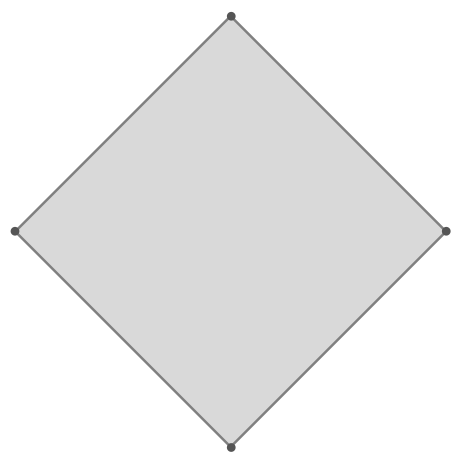
\includegraphics[width=0.3\columnwidth]{img/conv.png}
    \caption{Množina $C$ tvořená čtyřmi body a její konvexní obal $\textbf{conv }C$.}
    \label{img:conv}
\end{figure}

\chapter{Lineární programování}
%polyedr, formulace, dualita, ...
%příklad s řešením (dieta?)

\chapter{Semidefinitní programování}
%spektraedr, formulace, dualita, semidefinitní kužel, duální kužel, ...
%vektorové programování a jeho ekvivalence, formulace úloh

\chapter{Kuželové programování}
%jen stručně pro úplnost
